% Options for packages loaded elsewhere
\PassOptionsToPackage{unicode}{hyperref}
\PassOptionsToPackage{hyphens}{url}
\PassOptionsToPackage{dvipsnames,svgnames,x11names}{xcolor}
%
\documentclass[
  letterpaper,
  DIV=11,
  numbers=noendperiod]{scrartcl}

\usepackage{amsmath,amssymb}
\usepackage{iftex}
\ifPDFTeX
  \usepackage[T1]{fontenc}
  \usepackage[utf8]{inputenc}
  \usepackage{textcomp} % provide euro and other symbols
\else % if luatex or xetex
  \usepackage{unicode-math}
  \defaultfontfeatures{Scale=MatchLowercase}
  \defaultfontfeatures[\rmfamily]{Ligatures=TeX,Scale=1}
\fi
\usepackage{lmodern}
\ifPDFTeX\else  
    % xetex/luatex font selection
\fi
% Use upquote if available, for straight quotes in verbatim environments
\IfFileExists{upquote.sty}{\usepackage{upquote}}{}
\IfFileExists{microtype.sty}{% use microtype if available
  \usepackage[]{microtype}
  \UseMicrotypeSet[protrusion]{basicmath} % disable protrusion for tt fonts
}{}
\makeatletter
\@ifundefined{KOMAClassName}{% if non-KOMA class
  \IfFileExists{parskip.sty}{%
    \usepackage{parskip}
  }{% else
    \setlength{\parindent}{0pt}
    \setlength{\parskip}{6pt plus 2pt minus 1pt}}
}{% if KOMA class
  \KOMAoptions{parskip=half}}
\makeatother
\usepackage{xcolor}
\setlength{\emergencystretch}{3em} % prevent overfull lines
\setcounter{secnumdepth}{5}
% Make \paragraph and \subparagraph free-standing
\ifx\paragraph\undefined\else
  \let\oldparagraph\paragraph
  \renewcommand{\paragraph}[1]{\oldparagraph{#1}\mbox{}}
\fi
\ifx\subparagraph\undefined\else
  \let\oldsubparagraph\subparagraph
  \renewcommand{\subparagraph}[1]{\oldsubparagraph{#1}\mbox{}}
\fi


\providecommand{\tightlist}{%
  \setlength{\itemsep}{0pt}\setlength{\parskip}{0pt}}\usepackage{longtable,booktabs,array}
\usepackage{calc} % for calculating minipage widths
% Correct order of tables after \paragraph or \subparagraph
\usepackage{etoolbox}
\makeatletter
\patchcmd\longtable{\par}{\if@noskipsec\mbox{}\fi\par}{}{}
\makeatother
% Allow footnotes in longtable head/foot
\IfFileExists{footnotehyper.sty}{\usepackage{footnotehyper}}{\usepackage{footnote}}
\makesavenoteenv{longtable}
\usepackage{graphicx}
\makeatletter
\def\maxwidth{\ifdim\Gin@nat@width>\linewidth\linewidth\else\Gin@nat@width\fi}
\def\maxheight{\ifdim\Gin@nat@height>\textheight\textheight\else\Gin@nat@height\fi}
\makeatother
% Scale images if necessary, so that they will not overflow the page
% margins by default, and it is still possible to overwrite the defaults
% using explicit options in \includegraphics[width, height, ...]{}
\setkeys{Gin}{width=\maxwidth,height=\maxheight,keepaspectratio}
% Set default figure placement to htbp
\makeatletter
\def\fps@figure{htbp}
\makeatother

\KOMAoption{captions}{tableheading}
\makeatletter
\@ifpackageloaded{tcolorbox}{}{\usepackage[skins,breakable]{tcolorbox}}
\@ifpackageloaded{fontawesome5}{}{\usepackage{fontawesome5}}
\definecolor{quarto-callout-color}{HTML}{909090}
\definecolor{quarto-callout-note-color}{HTML}{0758E5}
\definecolor{quarto-callout-important-color}{HTML}{CC1914}
\definecolor{quarto-callout-warning-color}{HTML}{EB9113}
\definecolor{quarto-callout-tip-color}{HTML}{00A047}
\definecolor{quarto-callout-caution-color}{HTML}{FC5300}
\definecolor{quarto-callout-color-frame}{HTML}{acacac}
\definecolor{quarto-callout-note-color-frame}{HTML}{4582ec}
\definecolor{quarto-callout-important-color-frame}{HTML}{d9534f}
\definecolor{quarto-callout-warning-color-frame}{HTML}{f0ad4e}
\definecolor{quarto-callout-tip-color-frame}{HTML}{02b875}
\definecolor{quarto-callout-caution-color-frame}{HTML}{fd7e14}
\makeatother
\makeatletter
\makeatother
\makeatletter
\makeatother
\makeatletter
\@ifpackageloaded{caption}{}{\usepackage{caption}}
\AtBeginDocument{%
\ifdefined\contentsname
  \renewcommand*\contentsname{Table of contents}
\else
  \newcommand\contentsname{Table of contents}
\fi
\ifdefined\listfigurename
  \renewcommand*\listfigurename{List of Figures}
\else
  \newcommand\listfigurename{List of Figures}
\fi
\ifdefined\listtablename
  \renewcommand*\listtablename{List of Tables}
\else
  \newcommand\listtablename{List of Tables}
\fi
\ifdefined\figurename
  \renewcommand*\figurename{Figur}
\else
  \newcommand\figurename{Figur}
\fi
\ifdefined\tablename
  \renewcommand*\tablename{Table}
\else
  \newcommand\tablename{Table}
\fi
}
\@ifpackageloaded{float}{}{\usepackage{float}}
\floatstyle{ruled}
\@ifundefined{c@chapter}{\newfloat{codelisting}{h}{lop}}{\newfloat{codelisting}{h}{lop}[chapter]}
\floatname{codelisting}{Listing}
\newcommand*\listoflistings{\listof{codelisting}{List of Listings}}
\usepackage{amsthm}
\theoremstyle{definition}
\newtheorem{example}{Eksempel}[section]
\theoremstyle{definition}
\newtheorem{exercise}{Oppgave}[section]
\theoremstyle{remark}
\AtBeginDocument{\renewcommand*{\proofname}{Proof}}
\newtheorem*{remark}{Remark}
\newtheorem*{solution}{Solution}
\makeatother
\makeatletter
\@ifpackageloaded{caption}{}{\usepackage{caption}}
\@ifpackageloaded{subcaption}{}{\usepackage{subcaption}}
\makeatother
\makeatletter
\@ifpackageloaded{tcolorbox}{}{\usepackage[skins,breakable]{tcolorbox}}
\makeatother
\makeatletter
\@ifundefined{shadecolor}{\definecolor{shadecolor}{rgb}{.97, .97, .97}}
\makeatother
\makeatletter
\makeatother
\makeatletter
\makeatother
\ifLuaTeX
  \usepackage{selnolig}  % disable illegal ligatures
\fi
\IfFileExists{bookmark.sty}{\usepackage{bookmark}}{\usepackage{hyperref}}
\IfFileExists{xurl.sty}{\usepackage{xurl}}{} % add URL line breaks if available
\urlstyle{same} % disable monospaced font for URLs
\hypersetup{
  pdftitle={Ulikheter},
  pdfauthor={Elisabeth Engum},
  colorlinks=true,
  linkcolor={blue},
  filecolor={Maroon},
  citecolor={Blue},
  urlcolor={Blue},
  pdfcreator={LaTeX via pandoc}}

\title{Ulikheter}
\author{Elisabeth Engum}
\date{}

\begin{document}
\maketitle
\ifdefined\Shaded\renewenvironment{Shaded}{\begin{tcolorbox}[borderline west={3pt}{0pt}{shadecolor}, frame hidden, enhanced, sharp corners, boxrule=0pt, breakable, interior hidden]}{\end{tcolorbox}}\fi

\hypertarget{sec-utegnet}{%
\section{Ulikhetstegnet}\label{sec-utegnet}}

I delkapittelet om tallmengder, så vi på at vi kunne ha tallmengder som
består av elementer, eller som er gitt som åpne og/eller lukkete
intervaller.

\begin{tcolorbox}[enhanced jigsaw, colframe=quarto-callout-caution-color-frame, left=2mm, arc=.35mm, breakable, rightrule=.15mm, toprule=.15mm, leftrule=.75mm, opacityback=0, colback=white, bottomrule=.15mm]

Eksempel på elementer / liste: \(x\in\{-1, 2, 5\}\) som betyr at vi har
at x bare kan være lik \(-1\), \(2\) eller \(5\), og ingen andre verdier

Eksempel på åpne intervaller: \(x\in\langle 2, 4\rangle\) som betyr alle
tall på tallinjen som er større enn \(2\) og samtidig er mindre enn
\(4\)

Eksempel på lukkete intervaller: \(x\in\left[-1, 4\right]\) som betyr
alle tall på tallinjen som er større enn eller lik \(-1\) og samtidig
mindre enn eller lik \(4\).

\end{tcolorbox}

De åpne, halvåpne og lukkete intervallene kan også skrives med
ulikhetssymbol:

\begin{longtable}[]{@{}
  >{\raggedright\arraybackslash}p{(\columnwidth - 4\tabcolsep) * \real{0.1429}}
  >{\raggedright\arraybackslash}p{(\columnwidth - 4\tabcolsep) * \real{0.2857}}
  >{\raggedright\arraybackslash}p{(\columnwidth - 4\tabcolsep) * \real{0.5714}}@{}}
\caption{Ulikhetssymbolet (Merk at «gapet» alltid peker mot det største
tallet)}\tabularnewline
\toprule\noalign{}
\begin{minipage}[b]{\linewidth}\raggedright
Ulikhetssymbol
\end{minipage} & \begin{minipage}[b]{\linewidth}\raggedright
Leses som
\end{minipage} & \begin{minipage}[b]{\linewidth}\raggedright
Betyr
\end{minipage} \\
\midrule\noalign{}
\endfirsthead
\toprule\noalign{}
\begin{minipage}[b]{\linewidth}\raggedright
Ulikhetssymbol
\end{minipage} & \begin{minipage}[b]{\linewidth}\raggedright
Leses som
\end{minipage} & \begin{minipage}[b]{\linewidth}\raggedright
Betyr
\end{minipage} \\
\midrule\noalign{}
\endhead
\bottomrule\noalign{}
\endlastfoot
\(\lt\) & Mindre enn & Det som står på \textbf{venstre} siden av
symbolet er \textbf{mindre enn} det som står på høyre siden av
symbolet \\
\(\leq\) & Mindre enn eller lik & Det som står på \textbf{venstre} siden
av symbolet er \textbf{mindre enn eller lik} enn det som står på høyre
siden av symbolet \\
\(\gt\) & Større enn & Det som står på \textbf{venstre} siden av
symbolet er \textbf{større enn} det som står på høyre siden av
symbolet \\
\(\geq\) & Større enn eller lik & Det som står på \textbf{venstre} siden
av symbolet er \textbf{større enn eller lik} enn det som står på høyre
siden av symbolet \\
\end{longtable}

\hypertarget{ulikhetssymbolet-og-tallinjen}{%
\subsection{Ulikhetssymbolet og
tallinjen}\label{ulikhetssymbolet-og-tallinjen}}

\begin{figure}

{\centering 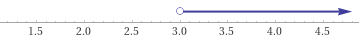
\includegraphics{Ulikheter_files/figure-pdf/fc7afa46-86dd-495e-9f39-4d4179823626-1-b51f81c9-1396-4a7a-9aed-a45061c5f20a.png}

}

\caption{Tallinje for x-verdier, og en linje som viser \(x>3\) (MÅ
BYTTES UT)}

\end{figure}

Det er to ulike måter vi kan skrive at vi har en tallmengde som består
av alle tall som er større enn 3.

\[ x\in\langle 3, \rightarrow\rangle\] \[x \gt 3 \]

Den siste linjen er også en \textbf{\emph{ulikhet}}.

\hypertarget{sec-ulikheter}{%
\section{Hva er ulikheter}\label{sec-ulikheter}}

I delkapittelet om likninger lærte dere ulike metoder for å finne ut når
et uttrykk på venste siden av likhetstegnet er lik uttrykket på høyre
siden av likhetstegnet. Et eksempel er å løse likningen

\[x^2-2x=3x-6\]

Denne likningen har to løsninger,
\(\underline{\underline{x\in\{2, 3\}}}\).

Men hva om vi ikke er på jakt etter når noe er helt likt? Kanskje vil vi
vite når noe er større enn eller mindre enn noe annet? Det kan være når
vi ønsker å finne ut hva som er billigst av to forskjellige
prismodeller.

\begin{tcolorbox}[enhanced jigsaw, colframe=quarto-callout-note-color-frame, title=\textcolor{quarto-callout-note-color}{\faInfo}\hspace{0.5em}{Ulikhet}, left=2mm, bottomtitle=1mm, coltitle=black, toprule=.15mm, leftrule=.75mm, opacityback=0, rightrule=.15mm, opacitybacktitle=0.6, breakable, toptitle=1mm, titlerule=0mm, arc=.35mm, bottomrule=.15mm, colbacktitle=quarto-callout-note-color!10!white, colback=white]

En ulikhet består av et ulikhetssymbol med tall eller uttrykk på hver
side

\end{tcolorbox}

\begin{tcolorbox}[enhanced jigsaw, colframe=quarto-callout-caution-color-frame, title={Eksempel}, left=2mm, bottomtitle=1mm, coltitle=black, toprule=.15mm, leftrule=.75mm, opacityback=0, rightrule=.15mm, opacitybacktitle=0.6, breakable, toptitle=1mm, titlerule=0mm, arc=.35mm, bottomrule=.15mm, colbacktitle=quarto-callout-caution-color!10!white, colback=white]

Mohammed og Turid skal bestille taxi, og vet ikke hva som er billigst av
1 Taxi AS eller ABC Taxi AS. Prisene er gitt som

\begin{longtable}[]{@{}lll@{}}
\toprule\noalign{}
& 1 Taxi AS & ABC Taxi AS \\
\midrule\noalign{}
\endhead
\bottomrule\noalign{}
\endlastfoot
Startpris & 104 kr & 112 kr \\
Pris per km & 10,80 kr & 10,50 kr \\
\end{longtable}

For hvilke avstander (i km) er ABC Taxi AS billigst?

\end{tcolorbox}

\begin{tcolorbox}[enhanced jigsaw, colframe=quarto-callout-caution-color-frame, left=2mm, arc=.35mm, breakable, rightrule=.15mm, toprule=.15mm, leftrule=.75mm, opacityback=0, colback=white, bottomrule=.15mm]

\textbf{Svar}\vspace{2mm}

Vi lar \(y\) være prisen for taxi-turen, og \(x\) antall kilometer. Da
får vi følgende uttrykk for prisene.

\begin{longtable}[]{@{}ll@{}}
\toprule\noalign{}
1 Taxi AS & ABC Taxi AS \\
\midrule\noalign{}
\endhead
\bottomrule\noalign{}
\endlastfoot
\(y = 104 + 10,80\cdot x\) & \(y = 112 + 10,50\cdot x\) \\
\end{longtable}

Hvis vi setter uttrykkene lik hverandre, så finner vi ut for hvilken
avstand det er lik pris. Men vi er jo på jakt etter når ABC Taxi AS er
billigst. Vi får altså en ulikhet, der vi skal finne ut når prisen på 1
Taxi er større enn prisen for ABC Taxi. Det kan vi skrive som følger:

\[ 104 + 10,80\cdot x > 112 + 10,50\cdot x\]

\end{tcolorbox}

Vi skal lære å løse sånne ulikheter her

\hypertarget{lineuxe6re-ulikheter-basert-puxe5-ndla}{%
\section{Lineære ulikheter (basert på
NDLA)}\label{lineuxe6re-ulikheter-basert-puxe5-ndla}}

En ulikhet inneholder gjerne en eller flere ukjente størrelser
symbolisert med bokstaver. Det er vanlig å bruke bokstaven \(x\) for den
ukjente når ulikheten har én ukjent størrelse.

Et eksempel er ulikheten
\begin{equation}\protect\hypertarget{eq-ulikhet1}{}{ x + 3 \geq 8 }\label{eq-ulikhet1}\end{equation}

Å \textbf{løse} en ulikhet går ut på å finne hvilke verdier \(x\) kan ha
for at ulikheten skal være sann. For eksempel, hvilke verdier av \(x\) i
ulikheten ovenfor gjør at \(x + 3\) blir lik eller større enn \(8\)?

\hypertarget{metode-for-uxe5-luxf8se-ulikheter}{%
\subsection{Metode for å løse
ulikheter}\label{metode-for-uxe5-luxf8se-ulikheter}}

Langt på vei kan vi løse ulikheter etter de samme prinsipper vi brukte
for å løse likninger.

\begin{itemize}
\item
  Hvis vi \textbf{adderer} det samme på begge sider av ulikhetstegnet,
  beholder vi den samme ulikheten mellom venstresiden og høyresiden.

  Siden \(5 \lt 9\), så er \(5\){\(+3\)} \(\lt 9\){\(+3\)}
\item
  Hvis vi \textbf{subtraherer} det samme tallet på begge sider av
  ulikhetstegnet, beholder vi den samme ulikheten mellom venstresiden og
  høyresiden.

  Siden \(9 \gt 5\), så er \(9\){\(-3\)} \(\gt 5\){\(-3\)}
\end{itemize}

Hvis vi bruker dette på ulikheten formel~\ref{eq-ulikhet1}, så får vi

\[\begin{align}\displaylines{x + 3 &\geq& 8 \\ x + 3 -3 &\geq& 8 - 3 \\ x &\geq& 5}\end{align}\]

\begin{tcolorbox}[enhanced jigsaw, colframe=quarto-callout-important-color-frame, title={Men hva med multiplikasjon og divisjon?}, left=2mm, bottomtitle=1mm, coltitle=black, toprule=.15mm, leftrule=.75mm, opacityback=0, rightrule=.15mm, opacitybacktitle=0.6, breakable, toptitle=1mm, titlerule=0mm, arc=.35mm, bottomrule=.15mm, colbacktitle=quarto-callout-important-color!10!white, colback=white]

La oss se på \(4 > 2\):

Hvis vi multipliserer hver side av ulikheten med 2, så får vi:

Venstre side: \(4\cdot 2 = 8\) Høyre side: \(2\cdot 2 = 4\)

Vi ser at ulikheten fortsatt er gyldig om vi multipliserer med et
positivt tall, fordi \(8>4\).

Men hva skjer om vi multipliserer med et \textbf{negativt tall} som for
eksempel \(-3\)?

Venstre side: \(4\cdot(-3)=-12\) Høyre side: \(2\cdot(-2)=-6\)

Men \(-12\) er jo mindre enn \(-6\), \(-12\) ligger lengre til venstre
på tallinjen enn \(-6\), og vi har fått at \(4\cdot(-3)<2\cdot(-3)\)!

\end{tcolorbox}

\begin{tcolorbox}[enhanced jigsaw, colframe=quarto-callout-note-color-frame, title=\textcolor{quarto-callout-note-color}{\faInfo}\hspace{0.5em}{Multiplikasjon og divisjon med negative tall}, left=2mm, bottomtitle=1mm, coltitle=black, toprule=.15mm, leftrule=.75mm, opacityback=0, rightrule=.15mm, opacitybacktitle=0.6, breakable, toptitle=1mm, titlerule=0mm, arc=.35mm, bottomrule=.15mm, colbacktitle=quarto-callout-note-color!10!white, colback=white]

Vi må alltid snu ulikhetstegnet når vi multipliserer eller dividerer med
negative tall

\end{tcolorbox}

\begin{itemize}
\item
  \textbf{Vi kan addere og subtrahere med samme tall på begge sider} i
  en ulikhet og forsatt beholde den samme ulikheten mellom venstre- og
  høyresiden.
\item
  \textbf{Vi kan multiplisere og dividere med samme positive tall på
  begge sider} i en ulikhet og fortsatt beholde den samme ulikheten
  mellom venstresiden og høyresiden.
\item
  \textbf{Vi må snu ulikhetstegnet hvis vi dividerer eller multipliserer
  med et negativt tall} på begge sider av ulikhetstegnet.
\end{itemize}

\begin{example}[Lineær
ulikhet]\protect\hypertarget{exm-Linulikhet1}{}\label{exm-Linulikhet1}

Vi løser ulikheten \(2x+3 < 4x+9\)

\[\require{cancel}\renewcommand{\CancelColor}{\red}\begin{align}\displaylines{2x + 3&<& 4x + 9 \\ 2x - 4x&<& 9 - 3 \\ -2x&<& 6 \\ \dfrac{\bcancel{-2}x}{\bcancel{-2}}&>& \dfrac{6}{-2} \\ x &>& -3}\end{align}\]

Svaret på en ulikhet blir en tallmengde, og vi kan oppgi svaret som
\[\underline{\underline{L\in\langle -3, \rightarrow \rangle}}\]

\end{example}

\begin{example}[Lineær
ulikhet]\protect\hypertarget{exm-Linulikhet2}{}\label{exm-Linulikhet2}

Løs ulikheten
\(\dfrac{x}{3}+\dfrac{1}{2} \leq \dfrac{x}{2}+\dfrac{1}{3}\)

\[\begin{align}\displaylines{\dfrac{x\cdot6}{3}+\dfrac{1\cdot6}{2} &\leq& \dfrac{x\cdot6}{2}+\dfrac{1\cdot6}{3} \\ 2x + 3 &\leq& 3x+2 \\ 2x-3x&\leq& 2-3 \\-x &\leq& -1 \\\dfrac{\bcancel{-}x}{\bcancel{-1}}&\geq& \dfrac{-1}{-1} \\ x &\geq& 1}\end{align}\]

Løsningsmengden for ulikheten er

\[\underline{\underline{L\in[1, \rightarrow \rangle}}\]

\end{example}

\hypertarget{luxf8se-ulikheter-med-cas}{%
\subsection{Løse ulikheter med CAS}\label{luxf8se-ulikheter-med-cas}}

Vi kan også løse ulikheter med CAS. Her kan vi enten skrive inn
ulikheten og trykke på knappen

\includegraphics{Ulikheter_files/figure-pdf/64440c9a-ee8e-4d8d-848c-75a06c2fa970-1-7bfe8851-df5a-404e-9f65-6532aead2c88.png}.

Da får vi denne løsningen:
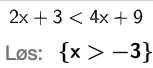
\includegraphics{Ulikheter_files/figure-pdf/64440c9a-ee8e-4d8d-848c-75a06c2fa970-3-9cbd829e-255c-49c5-83dc-df78e7bb2c7d.png}

Alternativt kan vi bruke kommandoordet ``Løs''.
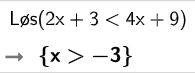
\includegraphics{Ulikheter_files/figure-pdf/64440c9a-ee8e-4d8d-848c-75a06c2fa970-2-8fbf58b9-721b-43b2-b963-4cb26026985a.png}

\hypertarget{oppgaver}{%
\section{Oppgaver}\label{oppgaver}}

\begin{exercise}[]\protect\hypertarget{exr-linulikhetOppgave1}{}\label{exr-linulikhetOppgave1}

Løs ulikhetene uten hjelpemidler, og deretter kontroller svaret ved å
løse ulikhetene med CAS.

\(x-3<5\)

\(2x+1<3\)

\(2x-4<x-4\)

\end{exercise}

\begin{exercise}[]\protect\hypertarget{exr-linulikhetOppgave2}{}\label{exr-linulikhetOppgave2}

Løs ulikhetene uten hjelpemidler, og deretter kontroller svaret ved å
løse ulikhetene med CAS.

\(5x-3<2x-6\)

\(6-5x\geq 6(1-x)\)

\(x-3\leq2(x+6)\)

\end{exercise}

\begin{exercise}[]\protect\hypertarget{exr-linulikhetOppgave3}{}\label{exr-linulikhetOppgave3}

Løs ulikhetene uten hjelpemidler, og deretter kontroller svaret ved å
løse ulikhetene med CAS.

\(3(x-5)<5(x-2)\)

\(1-x\leq 1+x\)

\(3(2x-3)<6x-9\)

\end{exercise}

\begin{exercise}[]\protect\hypertarget{exr-linulikhetOppgave4}{}\label{exr-linulikhetOppgave4}

Løs ulikhetene uten hjelpemidler, og deretter kontroller svaret ved å
løse ulikhetene med CAS.

\(\dfrac{x}{2}-\dfrac{x}{3} > \dfrac{1}{6}\)

\(\dfrac{5}{2}x+\dfrac{x}{3}-\dfrac{7}{4} \geq 3-\dfrac{x}{6}\)

\(\dfrac{3}{2}(2x - 3) < 9\left(\dfrac{x}{3} + \dfrac{1}{2}\right)\)

\end{exercise}



\end{document}
